\UseRawInputEncoding
\documentclass{beamer}
\usepackage[utf8]{inputenc}

\usetheme{Madrid}
\usecolortheme{default}
\usepackage{amsmath,amssymb,amsfonts,amsthm}
\usepackage{txfonts}
\usepackage{tkz-euclide}
\usepackage{listings}
\usepackage{adjustbox}
\usepackage{array}
\usepackage{tabularx}
\usepackage{gvv}
\usepackage{lmodern}
\usepackage{circuitikz}
\usepackage{tikz}
\usepackage{graphicx}
\usepackage{enumitem}

\setbeamertemplate{page number in head/foot}[totalframenumber]

\usepackage{tcolorbox}
\tcbuselibrary{minted,breakable,xparse,skins}



\definecolor{bg}{gray}{0.95}
\DeclareTCBListing{mintedbox}{O{}m!O{}}{%
  breakable=true,
  listing engine=minted,
  listing only,
  minted language=#2,
  minted style=default,
  minted options={%
    linenos,
    gobble=0,
    breaklines=true,
    breakafter=,,
    fontsize=\small,
    numbersep=8pt,
    #1},
  boxsep=0pt,
  left skip=0pt,
  right skip=0pt,
  left=25pt,
  right=0pt,
  top=3pt,
  bottom=3pt,
  arc=5pt,
  leftrule=0pt,
  rightrule=0pt,
  bottomrule=2pt,
  toprule=2pt,
  colback=bg,
  colframe=orange!70,
  enhanced,
  overlay={%
    \begin{tcbclipinterior}
    \fill[orange!20!white] (frame.south west) rectangle ([xshift=20pt]frame.north west);
    \end{tcbclipinterior}},
  #3,
}
\lstset{
    language=C,
    basicstyle=\ttfamily\small,
    keywordstyle=\color{blue},
    stringstyle=\color{orange},
    commentstyle=\color{green!60!black},
    numbers=left,
    numberstyle=\tiny\color{gray},
    breaklines=true,
    showstringspaces=false,
}
%------------------------------------------------------------
%This block of code defines the information to appear in the
%Title page
\title %optional
{2.10.79}
\date{September 30, 2025}

\author 
{Shreyas Goud Burra - EE25BTECH11051}
\begin{document}

\frame{\titlepage}

\begin{frame}{Question}
In a triangle $PQR$, let\\
$$\textbf{a}=\vec{QR},\, \textbf{b}=\vec{RP},\, \textbf{c}=\vec{PQ}$$
det \textbf{a} = 3,  det \textbf{b} = 4, and

$$\frac{\textbf{a}.(\textbf{c}-\textbf{b})}{\textbf{c}.(\textbf{a}-\textbf{b})}=\frac{\lvert \textbf{a}\rvert}{\lvert \textbf{a}\rvert+\lvert \textbf{b} \rvert}$$

then the value of $\lvert \textbf{a} \times \textbf{b} \rvert$ is \rule{1.5cm}{0.5mm}
\end{frame}

\begin{frame}{Given Information}
Let us find the solution theoretically first and then verify it computationally.\\
It is given that \textbf{a}, \textbf{b} and \textbf{c} are the sides of a triangle. This implies

\begin{align}
    \textbf{a}+\textbf{b}+\textbf{c} = \textbf{QR}+\textbf{RP}+\textbf{PQ} = 0
    \label{0.1}
\end{align}

It is also given that,
\begin{align}
    \lvert \textbf{a} \rvert=3\text{ and }\lvert \textbf{b} \rvert = 4
    \label{0.2}
\end{align}

\end{frame}
\begin{frame}{Solution}

Let the given equation,
\begin{align}
    \frac{\textbf{a}.(\textbf{c}-\textbf{b})}{\textbf{c}.(\textbf{a}-\textbf{b})}=\frac{\norm{\textbf{a}}}{\norm{\textbf{a}}+\norm{\textbf{b}}}
    \label{0.3}
\end{align}

This gives,

\begin{align}
    \frac{\textbf{a}.(\textbf{c}-\textbf{b})}{\textbf{c}.(\textbf{a}-\textbf{b})}=\frac{3}{7}
    \label{0.4}
\end{align}

\end{frame}

\begin{frame}
On further simplifying this gives us,

\begin{align}
    7(\textbf{a}^{\text{T}}\textbf{c}-\textbf{a}^{\text{T}}\textbf{b})=3(\textbf{c}^{\text{T}}\textbf{a}-\textbf{c}^{\text{T}}\textbf{b})
    \label{0.5}
\end{align}

\begin{align}
    4\textbf{a}^{\text{T}}\textbf{c}-7\textbf{a}^{\text{T}}\textbf{b}+3\textbf{c}^{\text{T}}\textbf{b}=0
    \label{0.6}
\end{align}

\end{frame}
\begin{frame}

On multiplying $\textbf{a}^{\textbf{T}}$ on both sides of \ref{0.1}

\begin{align}
    \textbf{a}^{\text{T}}\textbf{a}+\textbf{a}^{\text{T}}\textbf{b}+\textbf{a}^{\text{T}}\textbf{c}=0 \implies \textbf{a}^{\text{T}}\textbf{b}+\textbf{a}^{\text{T}}\textbf{c}=-9
    \label{0.7}
\end{align}

On multiplying $\textbf{b}^{\textbf{T}}$ on both sides of \ref{0.1}

\begin{align}
    \textbf{b}^{\text{T}}\textbf{a}+\textbf{b}^{\text{T}}\textbf{b}+\textbf{b}^{\text{T}}\textbf{c}=0 \implies \textbf{b}^{\text{T}}\textbf{a}+\textbf{b}^{\text{T}}\textbf{c}=-16
    \label{0.8}
\end{align}

\end{frame}
\begin{frame}
On solving the equations \ref{0.6}, \ref{0.7} and \ref{0.8}

\begin{align}
    \myvec{-7 & 3 & 4 \\ 1 & 0 & 1\\1 & 1 & 0} \myvec{\textbf{a}^\text{T}\textbf{b}\\\textbf{b}^\text{T}\textbf{c}\\\textbf{c}^\text{T}\textbf{a}\\}=\myvec{0\\-9\\-16}
    \label{0.9}
\end{align}

On using Gauss Jordan method to solve this
\begin{align}
    \myvec{\textbf{a}^\text{T}\textbf{b}\\\textbf{b}^\text{T}\textbf{c}\\\textbf{c}^\text{T}\textbf{a}\\}=\myvec{-7 & 3 & 4 &| & 0\\1& 0 & 1 & | &-9\\1&1&0&|&-16}
    \label{0.10}
\end{align}

\end{frame}
\begin{frame}
On doing $R_1\rightarrow R_1+8R_2$ and $R_3\rightarrow R_3-R_2$

\begin{align}
    \myvec{\textbf{a}^\text{T}\textbf{b}\\\textbf{b}^\text{T}\textbf{c}\\\textbf{c}^\text{T}\textbf{a}\\}=\myvec{1 & 3 & 12 &| & -72\\1& 0 & 1 & | &-9\\0&1&-1&|&-7}
    \label{0.11}
\end{align}

On doing $R_2\rightarrow R_2-R_1$

\begin{align}
    \myvec{\textbf{a}^\text{T}\textbf{b}\\\textbf{b}^\text{T}\textbf{c}\\\textbf{c}^\text{T}\textbf{a}\\}=\myvec{1 & 3 & 12 &| & -72\\0& -3 & -11 & | &63\\0&1&-1&|&-7}
    \label{0.12}
\end{align}
\end{frame}
\begin{frame}
On doing $R_1 \rightarrow R_1 + R_2$ and $R_3 \rightarrow R_3+\frac{1}{3}R_2$

\begin{align}
    \myvec{\textbf{a}^\text{T}\textbf{b}\\\textbf{b}^\text{T}\textbf{c}\\\textbf{c}^\text{T}\textbf{a}\\}=\myvec{1 & 0 & 1 &| & -9\\0& -3 & -11 & | &63\\0&0&-\frac{14}{3}&|&14}
    \label{0.13}
\end{align}

On doing $R_1\rightarrow R_1+\frac{3}{14}R_3$ and $R_2\rightarrow R_2-\frac{33}{14}R_3$

\begin{align}
    \myvec{\textbf{a}^\text{T}\textbf{b}\\\textbf{b}^\text{T}\textbf{c}\\\textbf{c}^\text{T}\textbf{a}\\}=\myvec{1 & 0 & 0 &| & -6\\0& -3 & 0 & | &30\\0&0&-\frac{14}{3}&|&14}
    \label{0.14}
\end{align}

\end{frame}
\begin{frame}

From this, we get,

\begin{align}
    \textbf{a}^\text{T}\textbf{b}=-6
    \label{0.15}
\end{align}

From the definition of cross product, and from \ref{0.15} we get,

\begin{align}
    \norm{\textbf{a} \times \textbf{b}}^2 = \norm{\textbf{a}}^2 \norm{\textbf{b}}^2-(\textbf{a}^\text{T}\textbf{b})^2 
    \implies \norm{\textbf{a} \times \textbf{b}}^2 = 4^2 . 3^2 -(-6)^2
    \label{0.16}
\end{align}

\end{frame}
\begin{frame}{Final Answer}

The final answer,

\begin{align}
    \norm{\textbf{a} \times \textbf{b}} = 6\sqrt{3}
\end{align}
\end{frame}


\begin{frame}[fragile]
\frametitle{C code}
\begin{lstlisting}
#include <stdio.h>
#include<math.h>

void cross(const double* a, const double* b, double* result) {
    result[0] = a[1]*b[2] - a[2]*b[1];
    result[1] = a[2]*b[0] - a[0]*b[2];
    result[2] = a[0]*b[1] - a[1]*b[0];
}

\end{lstlisting}
\end{frame}

\begin{frame}[fragile]
\frametitle{Python code}
\begin{lstlisting}

import numpy as np
import matplotlib.pyplot as plt
import ctypes
import os
import sys

a = np.array([3, 0, 0], dtype=np.float64)

y = 2
z = np.sqrt(12 - y**2)
b = np.array([-2, y, z], dtype=np.float64)  

axb = np.array([0, 0, 0], dtype=np.float64)

\end{lstlisting}
\end{frame}

\begin{frame}[fragile]
\frametitle{Python code}
\begin{lstlisting}



cross_lib = ctypes.CDLL('./cross.so')
cross_lib.cross.argtypes = [
        ctypes.POINTER(ctypes.c_double),
        ctypes.POINTER(ctypes.c_double),
        ctypes.POINTER(ctypes.c_double)
    ]

cross_lib.cross.restype = ctypes.c_double

cross=cross_lib.cross(
        a.ctypes.data_as(ctypes.POINTER(ctypes.c_double)),
        b.ctypes.data_as(ctypes.POINTER(ctypes.c_double)),
        axb.ctypes.data_as(ctypes.POINTER(ctypes.c_double))
    )
\end{lstlisting}
\end{frame}

\begin{frame}[fragile]
\frametitle{Python code}
\begin{lstlisting}

fig=plt.figure()
ax=fig.add_subplot(111, projection='3d')

ax.quiver(0, 0, 0, a[0], a[1], a[2], color='b', arrow_length_ratio=0.1)
ax.quiver(0, 0, 0, b[0], b[1], b[2], color='g', arrow_length_ratio=0.1)
ax.quiver(0, 0, 0, axb[0], axb[1], axb[2], color='r', arrow_length_ratio=0.1)

\end{lstlisting}
\end{frame}

\begin{frame}[fragile]
\frametitle{Python code}
\begin{lstlisting}

label = f'({a[0]}, {a[1]}, {a[2]})'
ax.text(a[0], a[1], a[2], s=label, color='b', fontsize=10)

label = f'({b[0]}, {b[1]}, {b[2]})'
ax.text(b[0], b[1], b[2], s=label, color='g', fontsize=10)

label = f'({axb[0]}, {axb[1]}, {axb[2]})'
ax.text(axb[0], axb[1], axb[2], s=label, color='r', fontsize=10)
\end{lstlisting}
\end{frame}

\begin{frame}[fragile]
\frametitle{Python code}
\begin{lstlisting}

ax.set_xlim([-10, 10])
ax.set_ylim([-10, 10])
ax.set_zlim([-10, 10])
plt.title('3D Projection of Vectors a, b, and a x b')
plt.savefig('/home/shreyas/GVV_Assignments/matgeo/2.10.79/figs/fig1.png')

plt.grid(True)
plt.show()
\end{lstlisting}
\end{frame}

\begin{frame}{3D Plot}
\begin{figure}[H]
    \centering
    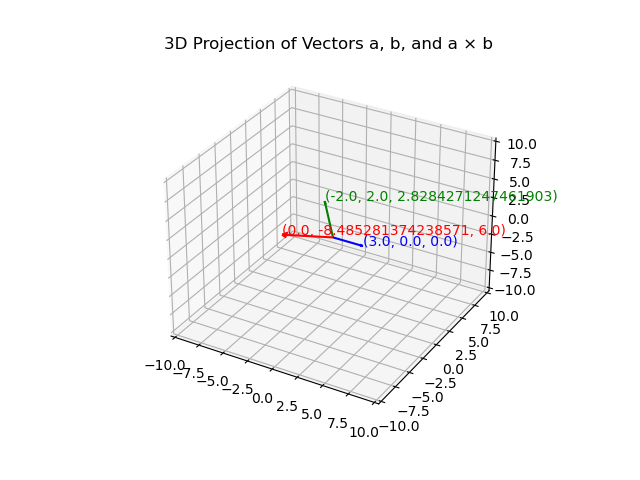
\includegraphics[width=0.8\columnwidth]{figs/fig1.png}
    \caption{3D Plot}
    \label{3D Plot}
\end{figure}
\end{frame}




\end{document}
